\documentclass[crop,tikz]{standalone}
\usepackage{tikz-qtree}


\begin{document}
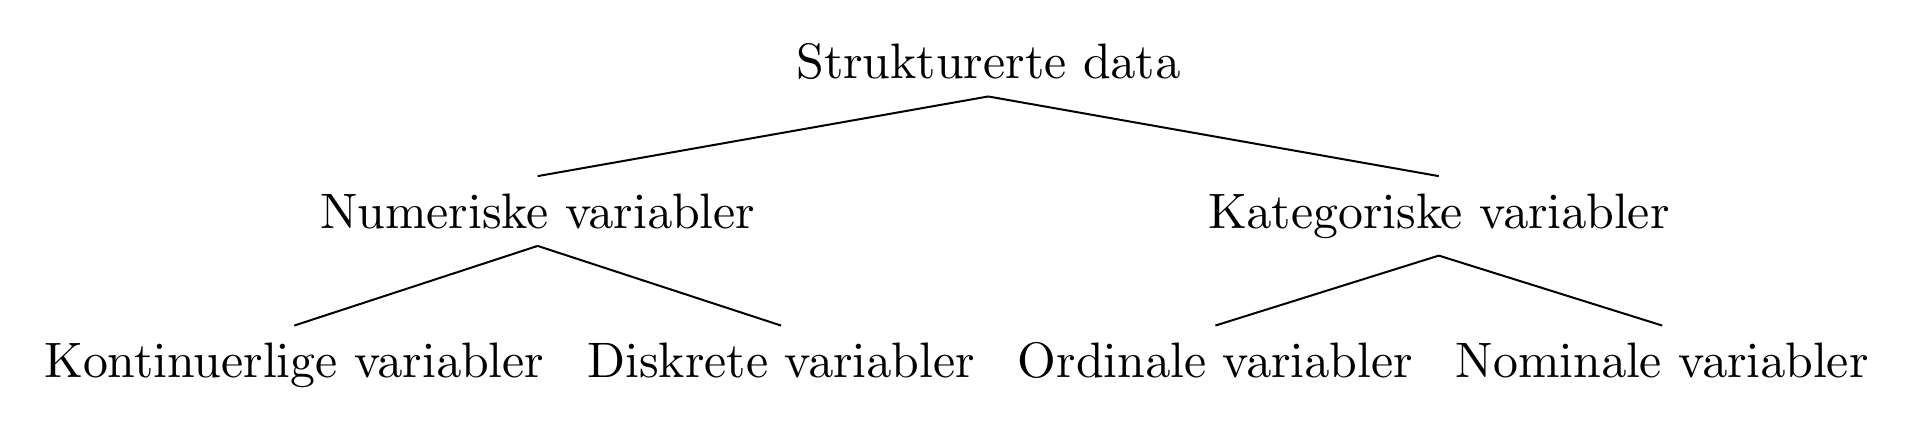
\begin{tikzpicture}[scale=1.8, transform shape]
\Tree 
    [.{Strukturerte data}
      [.{Numeriske variabler}
        [.{Kontinuerlige variabler} ]
        [.{Diskrete variabler} ]
    ]
      [.{Kategoriske variabler} 
        [.{Ordinale variabler} ]
        [.{Nominale variabler} ]
      ]
    ]
\end{tikzpicture}

\end{document}

%%% Local Variables:
%%% mode: latex
%%% TeX-master: t
%%% End:
